% Section and subsections will appear in the presentation overview
% and table of contents.
\section{Introduction}

\begin{frame}{Introduction}{}
  % applications of mobile robot navigation and problem description
  \begin{figure}
  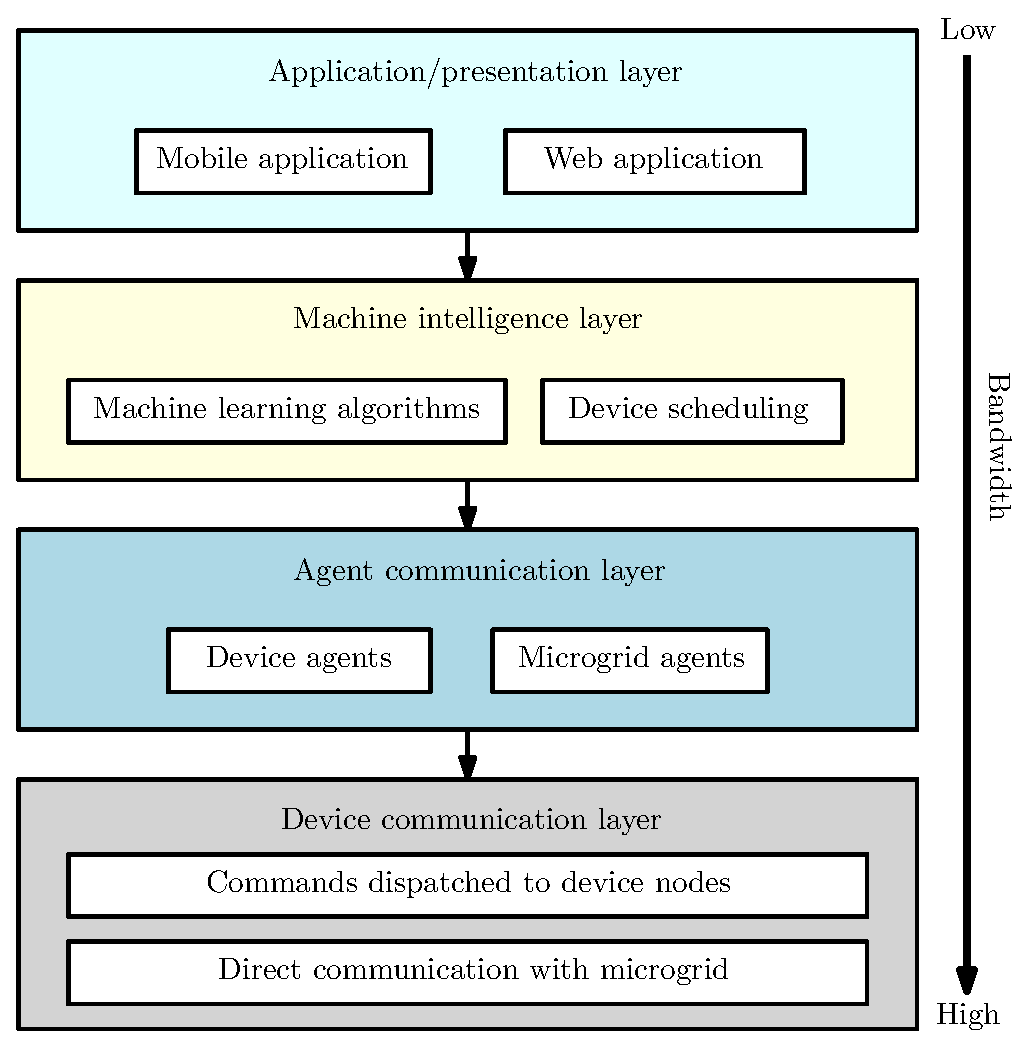
\includegraphics[scale=0.35]{figs/ipe/BEMS-softwareArchitecture}
  \end{figure}
\end{frame}

\begin{frame}{Introduction}{}
  % applications of mobile robot navigation and problem description
  \begin{figure}
  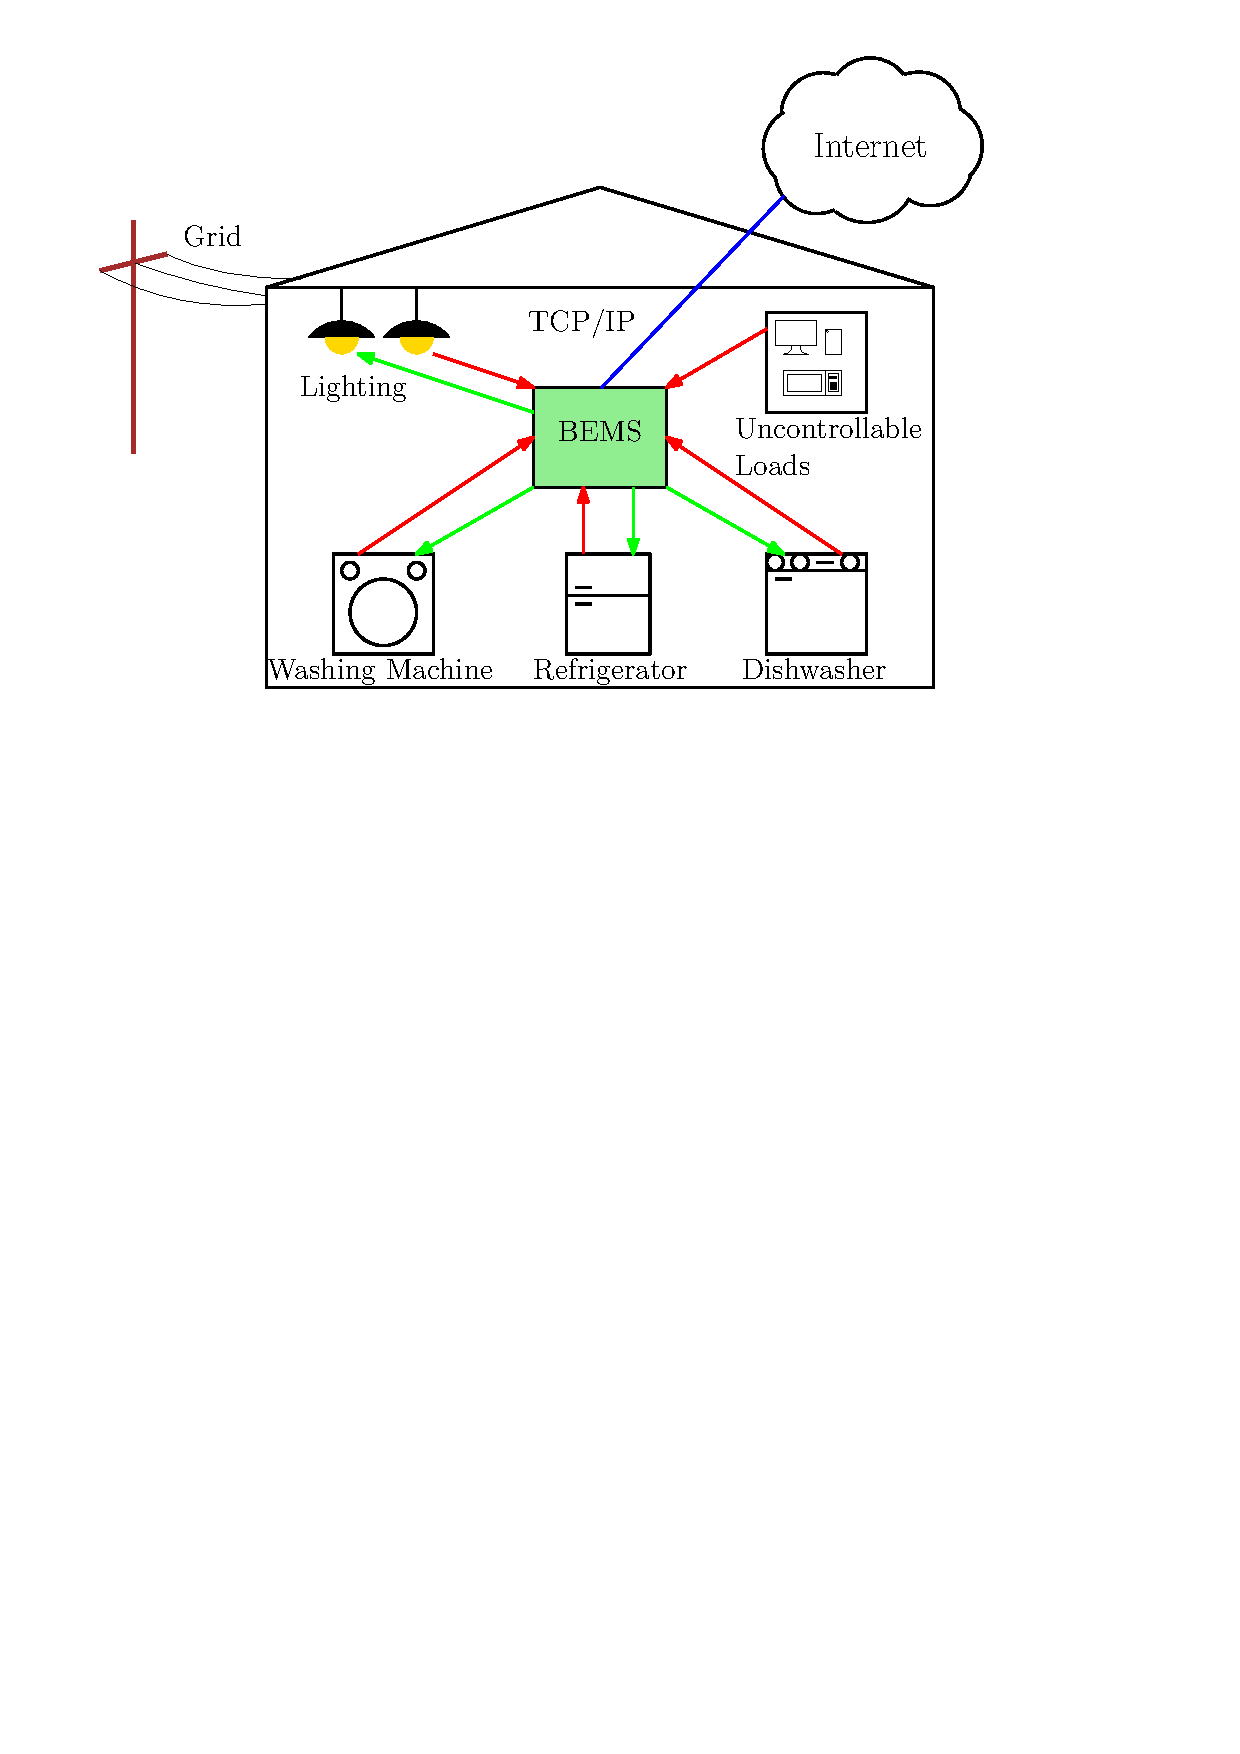
\includegraphics[scale=0.45]{figs/ipe/bemsdiagram}
  \end{figure}
\end{frame}


\section{Progress}
\begin{frame}{Progress}{}
\begin{itemize}
	\item Wrote an installation script with bash to fully automate installation of the software (\texttt{install.sh})
	\item Created a global settings python file to make project directories visible from any python module
	\item Developed a utilities module for miscellaneous utility functions
	\item Moved repository over to \texttt{BEMS-LauerMiah-GitHub}
\end{itemize}
\end{frame}

\subsection{Installation script}
\begin{frame}{Progress}{Installation script}
\begin{itemize}
	\item Assign the project directory variables
	\item Update Linux (\texttt{sudo apt-get update})
	\item Install python3-pip python3-venv xterm sqlite3	
	\item Delete the "venv" directory if it already exists
	\item Create a virtual environment name "venv"
	\item Activate the virtual environment
	\item Use the requirements.txt file to install all necessary dependencies
	\item Create a directories.pth file in the site-packages directory and add the directories to be added to the PYTHON\_PATH variable to the file
	\item Deactivate the virtual environment
\end{itemize}
\end{frame}

\subsection{Utilities module}
\begin{frame}{Progress}{Utilities module}
\begin{itemize}
	\item Contains a function for determining python version in format \texttt{python[major].[minor]}
	\item May add to it later as needed
	\item Could add a utility for connecting to databases to prevent boiler plate code from being written over and over again
\end{itemize}
\end{frame}

\section{Plans}
\begin{frame}{Plans}{}
\begin{itemize}
\item Implement the modal popup on the discovery page
\item Add devices to \texttt{ActiveDevices} database when discovered
\item Build page for controlling the WeMo Switch
\end{itemize}
\end{frame}



%%% Local Variables:
%%% mode: latex
%%% TeX-master: "../progressPresMain"
%%% End:
